\documentclass{article}

\usepackage{hyperref}
\usepackage{amssymb,amsfonts,amsmath,amsthm,pigpen,
,enumitem
,stmaryrd
,pifont
,hyphenat
,epigraph
,tikz
,etoolbox
,mparhack
,mathtools
,microtype
,lmodern
,datetime
,cite
,CJKutf8
,marvosym
,chessfss,
marvosym,wasysym,mathrsfs,afterpage,
tikz-cd,tikz}
%\usepackage[dvipsnames]{xcolor}
%\usepackage{enumerate,enumitem,tikz-cd,tikz,mathrsfs,graphicx,marvosym,wasysym,epigraph,afterpage}
%mathrsfs is for \mathscr, marvosym for \Coffeecup, graphicx for \heartsuit, wasysym is for \twonotes
%\usepackage[colorlinks=true, urlcolor=purple, linkcolor=RoyalBlue, citecolor=magenta, pdfborder={0 0 0}]{hyperref}
%\usepackage[document]{ragged2e}
%\usetikzlibrary{backgrounds}

\usepackage[all]{xypic}

\setlength\epigraphwidth{.6\textwidth}
%\setlength\epigraphrule{0pt}
\setlength{\parindent}{0pt}

\newcommand\blankpage{
    \null
    \thispagestyle{empty}
    \addtocounter{page}{-1}
    \newpage}

\newtheorem{thm}{Theorem}[section]
\newtheorem{cor}[thm]{Corollary}
\newtheorem{prop}[thm]{Proposition}
\newtheorem{lem}[thm]{Lemma}
\newtheorem{defn}[thm]{Definition}
\theoremstyle{definition} 
\newtheorem{exmp}[thm]{Example}
\newtheorem{rem}[thm]{Remark}

\newcommand{\Z}{\mathbb{Z}}
\newcommand{\Oo}{\mathcal{O}}
\newcommand{\ts}{\mathrm{ts}}
\newcommand{\tee}{\mathfrak{t}}
\newcommand{\orth}{\boxslash}
\newcommand{\per}{\Theta}
\newcommand{\pos}{\textnormal{Pos}}
\newcommand{\op}{\textnormal{op}}
\newcommand{\gr}{\Gamma}
\newcommand{\lex}{\times_{\textnormal{lex}}}

\DeclareMathOperator{\fib}{fib}
\DeclareMathOperator{\cofib}{cofib}

\begin{document}
\begin{titlepage}
\end{titlepage}




\subsection{The (he)art of gluing} The slice functor hides greater potential. Indeed, even if we don't have a morphism of $\mathbb{Z}$-posets (but just a $\mathbb{Z}$-equivariant map), then the slice functor can still be applied, obtaining a partially defined map. \\

Let $J$ be a $\Z$-toset, i.e., a totally ordered set together with a monotone action of $\Z$, that we will denote by $(n,x)\mapsto x+n$. Recall that a $J$-slicing on a stable $\infty$-category $\mathscr{D}$ is a morphism of $\Z$-posests $\tee\colon \Oo(J)\to \ts(\mathscr{D})$, where $\Oo(J)$ is the $\Z$-poset of the slicings of $J$ (i.e., the decompositions of $J$ into a disjoint union of a lower set $L$ and of an upper set $U$), and $\ts(\mathscr{D})$ is the $\Z$-poset of $t$-structures on $\mathscr{D}$.

Clearly, if $f\colon J\to J'$ is a morphism of $\Z$-tosets, then $f^{-1}\colon \{\text{subsets of $J'$}\}\to \{\text{subsets of $J$}\}$ induces a $\Z$-equivariant morphism of $\Z$-posets $f^{-1}\colon \Oo(J')\to \Oo(J)$, and so composition with $f^{-1}$ gives a morphism
\begin{align*}
f_*\colon J\text{-slicings on $\mathscr{D}$}&\to J'\text{-slicings on $\mathscr{D}$}\\
\tee&\mapsto \tee\circ f^{-1}.
\end{align*}
The slices of $f_*\tee$ are clearly given by $\mathscr{D}_{f_*\tee;\phi}=\mathscr{D}_{\tee;f^{-1}(\{\phi\})}$. Notice that, as $f$ is monotone, the subset $f^{-1}(\{\phi\})$ is an interval in $J$. It is immediate to see that $f_*$ restricts to a map
\begin{align*}
f_*\colon \text{Bridgeland $J$-slicings on $\mathscr{D}$}&\to \text{Bridgeland $J'$-slicings on $\mathscr{D}$}
\end{align*}
Namely, if $\mathcal{H}^\phi_{f_*\tee}(X)=0$ for every $\phi\in J'$ then $\mathcal{H}^{f^{-1}(\{\phi\})}_{\tee}(X)=0$ for every $\phi$ in $J'$. As we are assuming the $J$-slicing $\tee$ is a Bridgeland slicing, this implies that $\mathcal{H}^{\psi}_{\tee}(X)=0$ for every $\psi$ in $f^{-1}(\{\phi\})$, for every $\phi$. Therefore $\mathcal{H}^{\psi}_{\tee}(X)=0$ for every $\psi$ in $J$ and so, again by definition of Bridgeland slicing, $X=0$. Also, if $\mathcal{H}^\phi_{f_*\tee}(X)\neq 0$ then $\mathcal{H}^{f^{-1}(\{\phi\})}_{\tee}(X)\neq 0$ and so (again by the Bridgeland slicing condition) there exists at least an element $\psi$ in $f^{-1}(\{\phi\})$ such that $\mathcal{H}^{\psi}_{\tee}(X)\neq 0$. As the $J$-slicing $\tee$ is Bridgeland, the total of these $\psi$'s must be finite, so only for finitely many $\phi$ we can have such a $\psi$. In other words, the number of indices $\phi$ in $J'$ such that $\mathcal{H}^\phi_{f_*\tee}(X)\neq 0$ is finite.

Notice that, if $\tee$ is a Bridgeland slicing of $\mathscr{D}$, and $f\colon J\to J'$ is a morphism of $\Z$-tosets, then for any slicing $(L,U)$ of $J'$, the lower and the upper categories
$\mathscr{D}_{f_*\tee(L)}$ and $\mathscr{D}_{f_*\tee(U)}$ can be equivalently defined as
\begin{align*}
\mathscr{D}_{f_*\tee(L)}&=\langle \mathscr{D}_{\tee;\phi}\rangle_{f(\phi)\in L}\\
\mathscr{D}_{f_*\tee(U)}&=\langle \mathscr{D}_{\tee;\phi}\rangle_{f(\phi)\in U}
\end{align*}
where $\langle \mathscr{S}\rangle$ denotes the extension-closed subcategory of $\mathscr{D}$ generated by the subcategory $\mathscr{S}$.\footnote{
At some point it will be useful to recall Lemma 4.21 from ??:
Let $\mathscr{S}_1,\mathscr{S}_2$ be two subcategories of $\mathscr{D}$ with $\mathscr{S}_1\orth \mathscr{S}_2$, i.e., such that $\mathscr{D}(X_1,X_2)$ is contractible for any $X_1\in \mathscr{S}_1$ and any $X_2\in\mathscr{S}_2$. Then $\mathscr{S}_1\orth \langle\mathscr{S}_2\rangle$ and $\langle\mathscr{S}_1\rangle\orth \mathscr{S}_2$, and so $\langle\mathscr{S}_1\rangle\orth \langle\mathscr{S}_2\rangle$.}

The right hand sides of the above two expressions can clearly be defined for every morphism $f$ from $J$ to $J'$ (i.e., not necessarily monotone nor $\Z$-equivariant), and as soon as $f$ is $\Z$-equivariant, the assignment
\[
(L,U_\mapsto (\langle \mathscr{D}_{\tee;\phi}\rangle_{f(\phi)\in L},\langle \mathscr{D}_{\tee;\phi}\rangle_{f(\phi)\in U})
\]
is an equivariant morphism from $\mathcal{O}(J)$ to pairs of subcategories of $\mathscr{D}$. Clearly, when $f$ is not monotone there is no reason to expect that the pair $(\langle \mathscr{D}_{\tee;\phi}\rangle_{f(\phi)\in L},\langle \mathscr{D}_{\tee;\phi}\rangle_{f(\phi)\in U})$ forms a $t$-structure on $\mathscr{D}$. Yet, it interesting to notice that the condition that $f$ be monotone is only only sufficient in order to have this, and can indeed be relaxed.

\begin{defn}
Let $J$ and $J'$ be $\Z$-tosets, and let $f\colon J\to J'$ a map of $\Z$-sets (i.e., a $\Z$-equivariant map, not necessarily nondecreasing). A Bridgeland $J$-slicing $\tee$ of $\mathscr{D}$ is \emph{$f$-compatible}
if $f(\phi)>f(\psi)$ with $\phi\leq \psi$ implies $\mathscr{D}_{\tee; \phi}\orth \mathscr{D}_{\tee;\psi}$ and $\mathscr{D}_{\tee; \phi}\orth \mathscr{D}_{\tee;\psi}[1]$
\end{defn}

\begin{rem}
Clearly, if $f$ is monotone, then every $J$-slicing $\tee$ is order restoring as the condition `$f(\phi)>f(\psi)$ with $\phi\leq \psi$' is empty.
\end{rem}

\begin{lem}\label{is-t-structure}
Let $J$ and $J'$ be $\Z$-tosets, and let $f\colon J\to J'$ be a $\Z$-equivariant morphism of $\Z$-sets (i.e., not necessarily a monotone map) and let $\tee$ be a Bridgeland slicing of $\mathscr{D}$ which is $f$-compatible. Then, for any slicing $(L,U)$ of $J'$, the pair of subcategories
$(\langle \mathscr{D}_{\tee;\phi}\rangle_{f(\phi)\in L},\langle \mathscr{D}_{\tee;\phi}\rangle_{f(\phi)\in U})$ is a $t$-structure on $\mathscr{D}$.
\end{lem}
\begin{proof}
As $f$ is $\Z$-equivariant and $U+1\subseteq U$, we have
\begin{align*}
\langle \mathscr{D}_{\tee;\phi}\rangle_{f(\phi)\in U}[1]&=\langle \mathscr{D}_{\tee;\phi}[1]\rangle_{f(\phi)\in U}\\
&=\langle \mathscr{D}_{\tee;\phi+1}\rangle_{f(\phi)\in U}\\
&=\langle \mathscr{D}_{\tee;\phi+1}\rangle_{f(\phi+1)\in U+1}\\
&=\langle \mathscr{D}_{\tee;\phi}\rangle_{f(\phi)\in U+1}\\
&\subseteq \langle \mathscr{D}_{\tee;\phi}\rangle_{f(\phi)\in U}
\end{align*}
and similarly for the lower subcategory $\langle \mathscr{D}_{\tee;\phi}\rangle_{f(\phi)\in L}$. To show that 
\[
\langle \mathscr{D}_{\tee;\phi}\rangle_{f(\phi)\in U}\orth \langle \mathscr{D}_{\tee;\phi}\rangle_{f(\phi)\in L}
\]
it suffices to show that, if $f(\psi)\in L$ and $f(\phi)\in U$ then $\mathscr{D}_{\tee;\phi}\orth \mathscr{D}_{\tee;\psi}$. As $L\cap U=\emptyset$ we cannot have $\psi=\phi$, so either $\psi<\phi$ or vice versa. In the first case, $\mathscr{D}_{\tee;\phi}\orth \mathscr{D}_{\tee;\psi}$ by definition of Bridgeland $J$-slicing. In the second case, we have $\phi<\psi$ and $f(\phi)>f(\psi)$ as $f(\phi)\in U$ and  $f(\psi)\in L$. Therefore, since $\tee$ is $f$-compatible, $\mathscr{D}_{\tee;\phi}\orth\mathscr{D}_{\tee;\psi}$. Finally, we have to show that every object $X$ in $\mathscr{D}$ fits into a fiber sequence
\[
\xymatrix{
X_U\ar[r]\ar[d] & X\ar[d]\\
0\ar[r] & X_L
}
\]
with $X_L\in \langle \mathscr{D}_{\tee;\phi}\rangle_{f(\phi)\in L}$ and $X_U\in \langle \mathscr{D}_{\tee;\phi}\rangle_{f(\phi)\in U}$. As $\tee$ is a Bridgeland slicing, we have a factorization of the initial morphism $\mathbf{0} \to X$ of the form
\[
\mathbf{0}=X_0 \xrightarrow{\alpha_1} X_1\cdots \xrightarrow{\alpha_{{\bar\imath}}}X_{{\bar\imath}}\xrightarrow{\alpha_{{\bar\imath}+1}}X_{{\bar\imath}+1}\xrightarrow{}\cdots \xrightarrow{\alpha_n} X_n=X
\]
with $\mathbf{0} \neq \cofib(\alpha_i)=\mathcal{H}_{\tee}^{\phi_i}(X) \in \mathscr{D}_{\phi_i}$ for all $i = 1, \cdots, n$, with $\phi_i>\phi_{i+1}$. Let us now consider the sequence of symbols $L$ and $U$ obtained putting in the $i$-th place $L$ if $f(\phi_i)\in L$ and $U$ if $f(\phi_i)\in U$. If this sequence is of the form $(U,U,\dots,U,L,L,\dots,L)$, then there exists an index $\bar{\imath}$ such that
 $f(\phi_{i})\in U$ for $i\leq \bar{\imath}$ and $f(\phi_{i})\in L$ for $i>\bar{\imath}$ (with ${\bar\imath}=-1$ or $n$ when all of the $f(\phi_i)$ are in $L$ or in $U$, respectively). Then we can
consider the pullout diagram
\[
\xymatrix{
X_{{\bar\imath}}\ar[r]\ar[d]_{f_{L}}&0\ar[d]\\
X\ar[r]&\mathrm{cofib}(f_{L})
}\]
together with the factorizations
\[
\mathbf{0}=X_0 \xrightarrow{\alpha_1} X_1\cdots \xrightarrow{\alpha_{{\bar\imath}}}X_{{\bar\imath}} 
\]
and
\[
X_{{\bar\imath}}\xrightarrow{\alpha_{{\bar\imath}+1}}X_{{\bar\imath}+1}\xrightarrow{}\cdots \xrightarrow{\alpha_n} X_n=X.
\]
The first factorization shows that $X_{{\bar\imath}}\in \langle\cup_{i=0}^{{\bar\imath}}\mathscr{D}_{\phi_i}\rangle\subseteq \langle \mathscr{D}_{\tee;\phi}\rangle_{f(\phi)\in U}$ while the second factorization shows that $\mathrm{cofib}(f_{L})\in  \langle\cup_{i={\bar\imath}+1}^n\mathscr{D}_{\phi_i}\rangle\subseteq \langle \mathscr{D}_{\tee;\phi}\rangle_{f(\phi)\in L}$. So we are done in this case. Therefore, we are reduced to showing that we can always avoid a $(\dots,L,U,\dots)$ situation in our sequence of $L$'s and $U$'s. Assume we have such a situation. Then we have an index $i_0$ with $f(\phi_{i_0})\in L$ and $f(\phi_{{i_0}+1})\in U$. This in particular implies $f(\phi_{{i_0}+1})>f(\phi_{i_0})$ with $\phi_{{i_0}+1}<\phi_{i_0}$. As $\tee$ is $f$-compatible, this gives $\mathscr{D}_{\tee; \phi_{i_0+1}}\orth (\mathscr{D}_{\tee;\phi_{i_0}}[1])$. In particular, $\mathscr{D}(\mathcal{H}^{\phi_{i_0+1}}_{\tee}(X),\mathcal{H}^{\phi_{i_0}}_{\tee}(X)[1])$ is contractible. Now consider the pasting of pullout diagrams
\[
\xymatrix{X_{i_0-1}\ar[r]^{\alpha_{i_0}}\ar[d] & X_{i_0}\ar[r]^{\alpha_{i_0+1}}\ar[d] & X_{i_0+1}\ar[d]^{\gamma}\\
0\ar[r]&\mathcal{H}^{\phi_{i_0}}_{\tee}(X)\ar[d]\ar[r]&Y\ar[d]\ar[r] &0\ar[d]\\
&0\ar[r]&\mathcal{H}^{\phi_{i_0+1}}_{\tee}(X)\ar[r]&\mathcal{H}^{\phi_{i_0}}_{\tee}(X)[1].
}
\]
As the arrow $\mathcal{H}^{\phi_{i_0+1}}_{\tee}(X)\to \mathcal{H}^{\phi_{i_0}}_{\tee}(X)[1]$ factors through $0$, we have $Y=\mathcal{H}^{\phi_{i_0+1}}_{\tee}(X)\oplus \mathcal{H}^{\phi_{i_0}}_{\tee}(X)$ and the above diagram becomes
\[
\xymatrix{X_{i_0-1}\ar[r]^{\alpha_{i_0}}\ar[d] & X_{i_0}\ar[r]^{\alpha_{i_0+1}}\ar[d] & X_{i_0+1}\ar[d]^{\gamma}\\
0\ar[r]&\mathcal{H}^{\phi_{i_0}}_{\tee}(X)\ar[d]\ar[r]^-{\iota_2}&\mathcal{H}^{\phi_{i_0+1}}_{\tee}(X)\oplus \mathcal{H}^{\phi_{i_0}}_{\tee}(X)\ar[d]^{\pi_1}\ar[r] &0\ar[d]\\
&0\ar[r]&\mathcal{H}^{\phi_{i_0+1}}_{\tee}(X)\ar[r]&\mathcal{H}^{\phi_{i_0}}_{\tee}(X)[1],
}
\]
where $\iota_2$ and $\pi_1$ are the canonical inclusion and projection. Let $\beta\colon X_{i_0+1}\to \mathcal{H}^{\phi_{i_0}}_{\tee}(X)$ be the composition
\[
\beta\colon X_{i_0+1}\xrightarrow{\gamma} \mathcal{H}^{\phi_{i_0+1}}_{\tee}(X)\oplus \mathcal{H}^{\phi_{i_0}}_{\tee}(X)\xrightarrow{\pi_2} 
\mathcal{H}^{\phi_{i_0}}_{\tee}(X).
\]
Then we have a homotopy commutative diagram
\[
\xymatrix{
X_{i_0-1}\ar[r]^{\alpha_{i_0}}\ar[d]&X_{i_0}\ar[r]^{\alpha_{i_0+1}}\ar[d] & X_{i_0+1}\ar[d]^{\beta}\\
0\ar[r]&\mathcal{H}^{\phi_{i_0}}_{\tee}(X)\ar[r]^-{\mathrm{id}}&\mathcal{H}^{\phi_{i_0}}_{\tee}(X)
}
\]
(where only the left square is a pullout), and so the composition $\alpha_{i_0+1}\circ \alpha_{i_0}$ factors through the homotopy fiber of $\beta$. In other words, we have a homotopy commutative diagram
\[
\xymatrix{
X_{i_0-1}\ar[r]^{\alpha_{i_0}}\ar[d]_{\tilde{\alpha}_{i_0}}&X_{i_0}\ar[d]^{\alpha_{i_0+1}}\\
\fib(\beta)\ar[r]^{\tilde{\alpha}_{i_0+1}}&X_{i_0+1}\
}
\]
Writing $\tilde{X}_{i_0}=\fib(\beta)$, we get the pasting of pullout diagrams
\[
\xymatrix{X_{i_0-1}\ar[r]^{\tilde{\alpha}_{i_0}}\ar[d] & \tilde{X}_{i_0}\ar[r]^{\tilde{\alpha}_{i_0+1}}\ar[d] & X_{i_0+1}\ar[d]^{\gamma}\\
0\ar[r]&\mathcal{H}^{\phi_{i_0+1}}_{\tee}(X)\ar[d]\ar[r]^-{\iota_1}&\mathcal{H}^{\phi_{i_0+1}}_{\tee}(X)\oplus \mathcal{H}^{\phi_{i_0}}_{\tee}(X)\ar[d]_{\pi_2}\\
&0\ar[r]&\mathcal{H}^{\phi_{i_0}}_{\tee}(X).
}
\]
That is, by considering the factorization $X_{i_0-1}\xrightarrow{\tilde{\alpha}_{i_0}} \tilde{X}_{i_0}\xrightarrow{\tilde{\alpha}_{i_0+1}} X_{i_0+1}$ we have switched the cofibers with respect to the original factorization $X_{i_0-1}\xrightarrow{{\alpha}_{i_0}} {X}_{i_0}\xrightarrow{{\alpha}_{i_0+1}} X_{i_0+1}$. Therefore, writing $\tilde{\phi}_{i_0}=\phi_{i_0+1}$ and $\tilde{\phi}_{i_0+1}=\phi_{i_0}$, 
we now have  $f(\tilde{\phi}_{i_0})\in U$ and $f(\tilde{\phi}_{i_0+1})\in L$. That is, we have removed the $(\dots,L,U,\dots)$ situation from the position $i_0$, replacing it with a $(\dots,U,L,\dots)$ situation, while keeping all the labels $L,U$ before this positions unchanged. Repeating the procedure the needed number of times, we eventually get rid of all the $(\dots,L,U,\dots)$ situations.\footnote{This is somehow reminiscent of the `bubble sort' algorithm.}
\end{proof}

\begin{rem}\label{a-closer-look}
It follows from the proof of Lemma \ref{is-t-structure} that the objects $X_L$ and $X_U$ in the fiber sequence $X_U\to X\to X_L$ associated with the $t$-struture $(\langle \mathscr{D}_{\tee;\phi}\rangle_{f(\phi)\in L},\langle \mathscr{D}_{\tee;\phi}\rangle_{f(\phi)\in U})$ on $\mathscr{D}$ satisfy
\begin{align*}
X_L&\in \langle \mathscr{D}_{\tee;\phi};\quad f(\phi)\in L \text{ and }\mathcal{H}^\phi_\tee(X)\neq 0\rangle\\
X_U&\in \langle \mathscr{D}_{\tee;\phi};\quad f(\phi)\in U \text{ and }\mathcal{H}^\phi_\tee(X)\neq 0\rangle
\end{align*}
\end{rem}

\begin{lem}\label{slices}
For any $j\in J'$ we have
\[
\langle \mathscr{D}_{\tee;\phi}\rangle_{f(\phi)=j}=\langle \mathscr{D}_{\tee;\phi}\rangle_{f(\phi)\leq j}\cap \langle \mathscr{D}_{\tee;\phi}\rangle_{f(\phi)\geq j}.
\]
\end{lem}
\begin{proof}
Clearly, $\langle \mathscr{D}_{\tee;\phi}\rangle_{f(\phi)=j}\subseteq \langle \mathscr{D}_{\tee;\phi}\rangle_{f(\phi)\leq j}\cap \langle \mathscr{D}_{\tee;\phi}\rangle_{f(\phi)\geq j}$, therefore we only need to prove the converse inclusion. Let $\in \langle \mathscr{D}_{\tee;\phi}\rangle_{f(\phi)\leq j}\cap \langle \mathscr{D}_{\tee;\phi}\rangle_{f(\phi)\geq j}$. Then in particular 
$X\in \langle \mathscr{D}_{\tee;\phi}\rangle_{f(\phi)\geq j}$
and so there exists a factorization of the initial morphism $\mathbf{0} \to X$ of the form
\[
\mathbf{0}=X_0 \xrightarrow{\alpha_1} X_1\xrightarrow{\alpha_2}\cdots \xrightarrow{\alpha_{n-1}}X_{n-1}\xrightarrow{\alpha_n} X_n=X
\]
with $\mathbf{0} \neq \cofib(\alpha_i) \in \mathscr{D}_{\phi_i}$ with $f(\phi_i)\geq i$ for all $i = 1, \cdots, n$. As $((-\infty,j],(j,+\infty)$ is a slicing of $J'$, reasoning as in the proof of Lemma \ref{is-t-structure} we can arrange this factorization is such a way that $f(\phi_i)>j$ for $i\leq \bar{\imath}$ and $f(\phi_i)= j$ for $i>\bar{\imath}$. Therefore, again by reasoning as in the proof of Lemma \ref{is-t-structure} we get a fiber sequence of the form
\[
\xymatrix{
X_{>j}\ar[r]\ar[d] & X\ar[d]\\
0\ar[r]&X_{j}
}
\]
with $X_{>j}$ in $\langle \mathscr{D}_{\tee;\phi}\rangle_{f(\phi)>j}$ and $X_j$ in $\langle \mathscr{D}_{\tee;\phi}\rangle_{f(\phi)=j}$. This is in particular a fiber sequence of the form $X_{>j}\to X\to X_{\leq j}$, with $X_{\leq j}\in \langle \mathscr{D}_{\tee;\phi}\rangle_{f(\phi)\leq j}$. 
As $(\langle \mathscr{D}_{\tee;\phi}\rangle_{f(\phi)\leq j},\langle \mathscr{D}_{\tee;\phi}\rangle_{f(\phi)> j})$ is a $t$-structure on $\mathscr{D}$ by Lemma \ref{is-t-structure}, there is (up to equivalence) only one such a fiber sequence. And since $X\in \langle \mathscr{D}_{\tee;\phi}\rangle_{f(\phi)\leq j}$, this is the sequence $0\to X\xrightarrow{\mathrm{id}} X$. Therefore $X=X_j$.
\end{proof}

\begin{prop}
Let $f\colon J\to J'$ be a $\Z$-equivariant morphism of $\Z$-sets (i.e., not necessarily a monotone map) and let $\tee$ be a Bridgeland slicing of $\mathscr{D}$ which is $f$-compatible.  The map
\begin{align*}
f_!\tee\colon \Oo(J')&\to\ts(\mathscr{D})\\
(L,U)&\mapsto (\langle \mathscr{D}_{\tee;\phi}\rangle_{f(\phi)\in L},\langle \mathscr{D}_{\tee;\phi}\rangle_{f(\phi)\in U})
\end{align*}
defined by Lemma \ref{is-t-structure} is a Bridgeland $J'$-slicing of $\mathscr{D}$, with slices given by
\[
\mathscr{D}_{f_!\tee;j}=\langle \mathscr{D}_{\tee;\phi}\rangle_{f(\phi)=j}.
\]
\end{prop}
\begin{proof}
The map $f_!\tee$ is manifestly monotone and $\Z$-equivariant (see the first part of the proof of Lemma \ref{is-t-structure}), so it is a $J'$ slicing of $\mathscr{D}$, and its slices are given by $\mathscr{D}_{f_!\tee;j}=
%\mathscr{D}_{f_!\tee;\geq j}\cap \mathscr{D}_{f_!\tee;\leq j},
%\]
%and so by the subcategories $
\langle \mathscr{D}_{\tee;\phi}\rangle_{f(\phi)=j}$ by Lemma \ref{slices}. We are therefore left with showing that it is finite and discrete. Given an object $X$ in $\mathscr{D}$, let now $\{\phi_1,\dots,\phi_n\}$ be the indices in $J$ such that $\mathcal{H}^{\phi_i}_\tee(X)\neq 0$ and let $\{j_1,\dots,j_k\}$ the image of the set $\{\phi_1,\dots,\phi_n\}$ via $f$. Up to renaming, we can assume $j_1>j_{2}>\cdots>j_k$. Consider now the factorization
\[
\mathbf{0}=X_0 \xrightarrow{\alpha_1} X_1\xrightarrow{\alpha_2}\cdots \xrightarrow{\alpha_{k-1}}X_{k-1}\xrightarrow{\alpha_k} X_k=X
\]
of the initial morphism of $X$ associated to the decreasing sequence $j_1>j_2>\cdots>j_k$ by the $J'$-slicing $f_!\tee$. The cofibers of the morphisms $\alpha_{i}$ are the cohomologies
$\mathcal{H}^{(j_{i+1},j_{i}]}_{f_!\tee}(X)$ and, by Remark \ref{a-closer-look}, we have
\begin{align*}
\mathcal{H}^{(j_{i+1},j_{i}]}_{f_!\tee}(X)\in& \langle \mathscr{D}_{\tee;\phi};\quad f(\phi)\in (j_{i+1},j_{i}] \text{ and }\mathcal{H}^\phi_\tee(X)\neq 0\rangle\\
&=\langle \mathscr{D}_{\tee;\phi};\quad \phi\in\{\phi_1,\dots,\phi_n\}\text{ and } f(\phi)\in(j_{i+1},j_{i}]\rangle\\
&=\langle \mathscr{D}_{\tee;\phi};\quad \phi\in\{\phi_1,\dots,\phi_n\}\text{ and } f(\phi)=j_{i}\rangle\\
&\subseteq \langle \mathscr{D}_{\tee;\phi};\quad  f(\phi)=j_{i}\rangle=\mathscr{D}_{f_!\tee;j_{i}}.
\end{align*}
Therefore
\[
\mathcal{H}^{(j_i,j_{i-1}]}_{f_!\tee}(X)=\mathcal{H}^{j_i}_{f_!\tee}\mathcal{H}^{(j_i,j_{i-1}]}_{f_!\tee}(X)=\mathcal{H}^{j_i}_{f_!\tee}(X).
\]
This tells us that, if all the cohomologies $\mathcal{H}^{j}_{f_!\tee}(X)$ vanish, then also all the $\mathcal{H}^{(j_i,j_{i-1}]}_{f_!\tee}(X)$ vanish, and so $X=0$. Finally, if $\tilde{j}\notin\{j_1,\dots,j_k\}$, then there exists an index $i$ such that $j_{i+1}<\tilde{j}<j_{i}$ and so $(j_{i+1},\tilde{j}]\cap \{j_1,\dots,j_k\}=\emptyset$. The above argument then shows that
\[
\mathcal{H}^{(j_{i+1},\tilde{j}]}_{f_!\tee}(X)\in\langle \mathscr{D}_{\tee;\phi};\quad \phi\in\{\phi_1,\dots,\phi_n\}\text{ and } f(\phi)\in(j_{i+1},\tilde{j}]\rangle=\{\mathbf{0}\}.
\]
It follows that 
\[
\mathcal{H}^{\tilde{j}}_{f_!\tee}(X)=\mathcal{H}^{\tilde{j}}_{f_!\tee}\mathcal{H}^{(j_{i+1},\tilde{j}]}_{f_!\tee}(X)=\mathcal{H}^{\tilde{j}}_{f_!\tee}(0)=0,
\]
for every $\tilde{j}\notin \{j_1,\dots,j_k\}$. So in particular, for any $X\in \mathscr{D}$, the cohomologies $\mathcal{H}^{j}_{f_!\tee}(X)$ are possibly nonzero only for finitely many indices $j$. 
\end{proof}


Let now $J_1$ and $J_2$ be two $\mathbb{Z}$-tosets, and let $J_1 \lex J_2$ and $J_2 \lex J_1$ the two $\Z$-tosets obtained by considering the lexicogaphic order on the products $J_1\times J_2$ and $J_2\times J_1$, respectively, and the diagonal $\Z$ action. The following lemma is immediate.
\begin{lem}
The exchange map
\begin{align*}
e\colon J_1\times J_2&\to J_2\times J_1\\
(j_1,j_2)&\mapsto (j_2,j_1)
\end{align*}
is $\Z$-equivariant.
\end{lem}

\begin{defn}
Let $J_1$ and $J_2$ be $\Z$-tosets. A Bridgeland $J_1 \lex J_2$-slicing $\tee$ of $\mathscr{D}$ is said to be \emph{gluable} if it is $e$-compatible, where $e \colon J_1 \times J_2 \to J_2 \times J_1$ is the exchange map. 
\end{defn}

\begin{exmp} Let $J_1=\{0,1\}$ with the trivial $\Z$-action and let $J_2=\Z$ with the standard translation $\Z$-action.  Then a $J_1\lex J_2$-slicing $\tee$ on $\mathscr{D}$ is the datum of a semiorthogonal decomposition $(\mathscr{D}_0,\mathscr{D}_1)$ of $\mathscr{D}$ toghether with $t$-structures $\tee_i$ on $\mathscr{D}_i$. Spelling out the definiton, one sees that the $\{0,1\}\lex \Z$-slicing $\tee$ is gluable if and only if 
$\mathscr{D}_{0;\geq 0}\orth \mathscr{D}_{1;-1}$ and $\mathscr{D}_{0;\geq 0}\orth \mathscr{D}_{1;0}$. When this happens, the glued slicing $e_!\tee$ is a $\Z\lex\{0,1\}$ slicing on $\mathscr{D}$, i.e., is the datum of a bounded $t$-structure on $\mathscr{D}$ together with a torsion theory on its heart. More precisely, the heart of $e_!\tee$ is the full $\infty$-subcategory $\mathscr{D}^{\heartsuit_{e_!\tee}}$ of $\mathscr{D}$ on thise objects $X$ that fall into fiber sequences of the form $X_1\to X\to X_0$ with $X_i\in \mathscr{D}_i^\heartsuit$, while the torsion theory on $\mathscr{D}^{\heartsuit_{e_!\tee}}$ is
$(\mathscr{D}_0^{\heartsuit},\mathscr{D}_1^{\heartsuit})$, i.e., precisely the pair of hearts of the two subcategories in the semiorthogonal decomposition.
\end{exmp}


{\Huge -fino a qui-}


\begin{rem}
  In {\color{red}ref: BBD} the authors consider a process consisting in gluing $t$-structures on a pair of triangulated categories to obtain a $t$-structure on a third one. In their setting, the three categories are linked by an abstraction of the Grothendieck's six-functors formalism. However, the latter is more or less equivalent to the datum of a semiorthogonal decomposition (i.e., a $\{0,1 \}$-slicing, where $\{0,1 \}$ is the toset with two elements and trivial $\Z$-action) on the third category so that the input of the two (bounded) $t$-structures gives rise to a gluable $\{0,1\} \lex \Z$-slicing $\tee$. Then the $\Z \lex \{0,1 \}$-slicing $e_! \tee$ is just the new glued $t$-structure together with the natural torsion pair on its heart. This explains our terminology and links the language of the present paper to the classical theory of $t$-structures. 
\end{rem}

To motivate the next section, consider the following isomorphism fo $\Z$-tosets:
  \begin{align*}
     \Z \lex \Z &\to \Z \lex \Z_{\textnormal{free}} \\
   (n,m) & \mapsto (n,m-n)  
  \end{align*}


  ...continua ...
  
\begin{lem}
  Let $p \colon J \to \Oo(J')^\op$ be a monotone map. Then $$\gr(p)=\{ (n,j) \in J \times J'; \quad j \in U_{p(n)} \}.$$
  is an upper set of $J \times J'$ with the product order.
\end{lem}

\begin{proof}
Pick $(n,j) \leq (m,k)$ in $J \times J'$ and suppose $(n,j) \in \gr(p)$. Then $j \in p(n) \in \Oo(J')$ and since $j \leq k$ we have that $k \in p(n)$. But  $n \leq m$ and $p$ is monotone, and thus $p(n) \subseteq p(m)$. This gives $k \in p(m)$, as desired. \\
\end{proof}


\begin{prop}
  The map 
  \begin{align*}
 \gr \colon \pos(J,\Oo(J')^\op)&\to \Oo(J \times J')\\
   p & \mapsto (J \times J' \setminus \gr(p), \gr(p))  
  \end{align*}
is an isomorphism of $\Z$-posets, where $J \times J'$ carries the product order. 
\end{prop}

\begin{proof}
  Pick and upper set $U$ of $J \times J'$ and set, for $n \in J$ $$p_U(n)=\{ j \in J'; \quad  (n,j) \in U \}.$$
 Then the map
   \begin{align*}
   \Oo(J \times J') &\to \pos(J,\Oo(J')^\op) \\
  (L,U) & \mapsto p_U
  \end{align*}
  is inverse to $\gr(p)$ by a straightforward check. 
\end{proof}

\begin{defn}
A \emph{perversity} on $J$ is a monotone map $p \colon \Z \to \Oo(J)^\op$ such that $$p(n)-n \leq p(m) -m$$
whenever $m \leq n$ in $\Z$. The set of all perversities on $J$ will be denoted $\per(J)$. 
\end{defn}

\begin{rem}
We can give $\per(J)$ the structure of a $\Z$-poset via the incluion $\per(J) \subseteq \pos(\Z,\Oo(J)^\op)$. In general, it will not be totally ordered. However, by taking joins and meets pointwise $\per(J)$ becomes a distributive lattice. 
\end{rem}

\begin{rem}
Considering the obvious isomoprhism $\Z \simeq \Oo(\Z)^\op$ a perversity over $\mathbb{Z}$ is just a \textit{monotone and comonotope perversity} in the sense of {\color{red} referenza, tipo bezrukavnikov o BBD}. 
\end{rem}










{\Huge fino a qui 2}

%\begin{prop}\label{pipp}
%Let $J \overset{f}{\longrightarrow} J'$ be a a $\mathbb{Z}$-equivariant map (not necessarily increasing) between $\mathbb{Z}$-posets, $\mathscr{P}$ a $J$-slicing on $\mathscr{D}$. Suppose that $\mathscr{P}_{\psi} \subseteq \mathscr{P}_{\phi}^{\perp}$ whenever one of the following conditions holds: 
%\begin{enumerate}[label=(\alph*)]
%\item $f(\phi) > f(\psi)$
%\item $f(\phi) + 1 > f(\psi)$ and $\phi +1 < \psi$
%\end{enumerate}
%Then $$(f_{\textnormal{\Libra}}(\mathscr{P}))_{\phi}=\mathscr{P}_{f^{-1}(\phi)}$$
%defines a $J'$-slicing on $\mathscr{D}$.
%\end{prop}
%
%\begin{proof}
%Part \textit{(1)} of definition of slicing follows from $\mathbb{Z}$-equivariance of $f$, while part \textit{(2)} follows from condition \textit{(a)} above. Pick $0 \not = X \in \mathscr{D}$ and consider its Postnikov tower with respect to $\mathscr{P}$: $$0=Y_0 \overset{\beta_1}{\longrightarrow} \cdots \overset{\beta_n}{\longrightarrow} Y_n=X$$
%with $\textnormal{cone}(\beta_i)=H_{\mathscr{P}}^{\phi_i}(X)$. Going from left to right, if we encounter an $i$ so that $f(\phi_{i+1}) > f(\phi_i)$ then by condition \textit{(b)} $$\textnormal{Hom}_{\mathscr{D}}(H_{\mathscr{P}}^{\phi_{i+1}}(X),H_{\mathscr{P}}^{\phi_i}(X)[1])=0$$
%
%Using \hyperref[g]{\textbf{Proposition \ref*{g}}} and the \hyperref[s]{\textbf{$3 \times 3$ Lemma}}, we can complete the identity of $Y_i$ to get a diagram: 
%\begin{center}
%\begin{tikzcd}[ampersand replacement=\&]
%H_{\mathscr{P}}^{\phi_{i+1}}(X)[-1] \arrow{r} \arrow{d} \& Y_i \arrow{r} \arrow{d}{1} \& Y_{i+1} \arrow{r} \arrow{d} \& H_{\mathscr{P}}^{\phi_{i+1}}(X)[1]\arrow{d} \\
%Y_{i-1} \arrow{d} \arrow{r} \& Y_i \arrow{r} \arrow{d} \& H_{\mathscr{P}}^{\phi_i}(X) \arrow{r} \arrow{d} \& Y_{i-1}[1] \arrow{d} \\
%A \arrow{r} \arrow{d} \& 0 \arrow{r} \arrow{d} \& A[1] \arrow{r} \arrow{d} \& A[1] \arrow{d}  \\
%H_{\mathscr{P}}^{\phi_{i+1}}(X) \arrow{r}  \&  Y_i[1] \arrow{r} \& Y_{i+1}[1] \arrow{r} \&  H_{\mathscr{P}}^{\phi_{i+1}}(X)[1]
%\end{tikzcd}
%\end{center}
%
%We then replace $\beta_i$ with $Y_{i-1} \longrightarrow A$ and $\beta_{i+1}$ with $A \longrightarrow Y_{i+1}$. Iterating this process\footnote{This is somehow reminiscent of the 'bubble sort' algorithm.}, we get a factorization $$0=Z_0 \overset{\gamma_1}{\longrightarrow} \cdots \overset{\gamma_n}{\longrightarrow} Z_n=X$$
%with $\textnormal{cone}(\gamma_i)=H_{\mathscr{P}}^{\phi_{k_i}}(X)$ for some $k_i$ and $f(\phi_i) \ge f(\phi_{i+1})$ for all $i$. To get a factorization with the strict latter inequality we use the same argument as in the proof of \hyperref[af]{\textbf{Proposition \ref*{af}}}.
%\end{proof}
%
%The above proof also shows that, in the same hypotheses and notation, $(f_{\textnormal{\Libra}}(\mathscr{P}))_{\phi}$ consists of objects $X \in \mathscr{D}$ so that $H_{\mathscr{P}}^{\psi}(X)=0$ for $ f(\psi) \not = \phi$. Also, \hyperref[aae]{\textbf{Proposition \ref*{aae}}} holds when $f$ is bijective.\\

\begin{defn}
Let $\mathfrak{t}$ be a bounded t-structure on $\mathscr{D}$. An abelian $\mathbb{Z}$-slicing $\mathscr{P}$ on $\heartsuit_{\mathfrak{t}}$ is called:
\begin{itemize}
\item \textbf{perverse filtration} if $\mathscr{P}_{\psi}[n] \subseteq \mathscr{P}_{\phi}^{\perp}$ for $n < \phi - \psi$
\item \textbf{grading filtration} if it is a perverse filtration and $\mathscr{P}_{\psi}[n] \subseteq \mathscr{P}_{\phi }^{\perp}$ for $2 \le n = \phi - \psi$ 
\item \textbf{mixed filtration} if $\mathscr{P}_{\psi}[n] \subseteq \mathscr{P}_{\phi }^{\perp}$ for $n > \psi - \phi$ 
\end{itemize} 
\end{defn}

The following implications hold: 
$$\textnormal{mixed} \implies \textnormal{grading} \implies \textnormal{perverse} $$
{\color{red}proof that mixed implies grading: suppose $n< \phi - \psi$. By definition of slicing, the vanishing is automatic for $n \le 0$ and we can thus assume $n>0$. But then $n>0>-n>\psi-\phi$ and the required vanishing now follows from the definition of mixed filtration. The same argument also works for $2 \le n = \phi - \psi$}. \\
Clearly, a torsion pair on $\heartsuit_{\mathfrak{t}}$ (seen as an abelian $\mathbb{Z}$-slicing via the inclusion $[1] \subseteq \mathbb{Z}$) is always a grading filtration {\color{red}(proof: it follows from the fact that $\mathscr{P}_{\phi}[n]=0$ for $\phi \not = 0,1$ and thus the only nontrivial case is $n=0, \phi=1, \psi=0$. The Hom-vanishing then follows from the definition of torsion pair)}. Historically, grading filtrations first appeared in \cite{ekh} under the name of 'radical filtrations', while mixed filtrations are covered in the last section of \cite{kos}.

\begin{defn}
A map $\mathbb{Z} \overset{p}{\longrightarrow} \mathbb{Z}$ is called \textbf{perversity} if it is a monotone contraction, i.e. if $$0 \le p(\phi) - p(\psi) \le \phi - \psi$$ 
whenever $\phi \ge \psi$  in $\mathbb{Z}$. \\
We denote $\Xi$ the set of perversities. 
\end{defn}

Clearly, $\Xi$ definies a $\mathbb{Z}$-poset which is not totally ordered. However, it is a distributive lattice: we have meets and joins given by: $$(p\land q)(\phi)=\min\{p(\phi), q(\phi) \}$$ $$(p\lor q)(\phi)=\max\{p(\phi), q(\phi) \}$$
Indeed, if we place on $\mathbb{Z}\times \mathbb{Z}$ the product order, we have an isomorphism of $\mathbb{Z}$-posets $$\Xi^{\textnormal{op}}=O(\mathbb{Z}\times \mathbb{Z})\setminus \{ \emptyset, \mathbb{Z} \times \mathbb{Z} \} $$
given by sending the zero perversity to $A=\{ (\phi,\psi) \}_{\phi \ge 0} $ and the identity to $B=\{ (\phi,\psi) \}_{\psi \ge 0}$ ($B+i$ and $A+i$ with $i \in \mathbb{Z}$ generate the latter as a complete lattice). Considering the canonical embedding $\mathbb{Z} \hookrightarrow \mathbb{Z}  \subseteq O(\mathbb{Z} \times \mathbb{Z})$ we get a sublattice of $\Xi$ depicted as 

 \begin{center}
      \begin{tikzpicture}
        \draw (-2,-2) -- (-1,-1) -- (0,0) -- (1,-1) -- (2,-2);
        \draw (-1,-1) -- (0,-2) -- (1,-1);
        \draw (-3,-3) -- (-2,-2) -- (-1,-3) -- (0,-2) -- (1,-3) -- (2,-2) -- (3,-3);
       \node at (0,1) {$\vdots$};
       \node[circle, draw, fill=black, inner sep=0pt, minimum width=4pt] at (0,0) {};
       \node[circle, draw, fill=black!50, inner sep=0pt, minimum width=4pt] at (-1,-1) {};
       \node[circle, draw, fill=black!50, inner sep=0pt, minimum width=4pt] at (1,-1) {};
       \node[circle, draw, fill=black!50, inner sep=0pt, minimum width=4pt] at (0,-2) {};
       \node[circle, draw, fill=black!50, inner sep=0pt, minimum width=4pt] at (-2,-2) {};
       \node[circle, draw, fill=black!50, inner sep=0pt, minimum width=4pt] at (2,-2) {};
       \node[circle, draw, fill=black!50, inner sep=0pt, minimum width=4pt] at (-3,-3) {};
       \node[circle, draw, fill=black!50, inner sep=0pt, minimum width=4pt] at (-1,-3) {};
       \node[circle, draw, fill=black!50, inner sep=0pt, minimum width=4pt] at (1,-3) {};
       \node[circle, draw, fill=black!50, inner sep=0pt, minimum width=4pt] at (3,-3) {};
       \node at (0,-4) {$\vdots$};
      \end{tikzpicture}
    \end{center}
This induces the 't-tree' described in \cite{matti}, as discussed below in a far-reaching generality. By the other hand, each square above contains moreover a copy of the Young lattice
 \begin{center}
      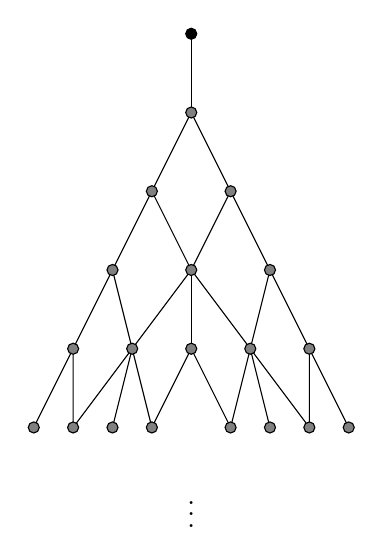
\begin{tikzpicture}[nodes={circle, draw, fill=black!50, inner sep=0pt, minimum width=4pt}]
              \draw (2,-4) -- (1.5,-3) -- (1,-2) -- (0.5,-1) -- (0,0) -- (-0.5,-1) -- (-1,-2) -- (-1.5,-3) -- (-2,-4);
        \draw (1.5,-3) -- (1.5,-4) -- (0.75,-3) -- (0,-2) -- (-0.75,-3) -- (-1.5,-4) -- (-1.5,-3);
        \draw  (1,-4) -- (0.75,-3) -- (0.5,-4) -- (0,-3) -- (-0.5,-4) -- (-0.75,-3) -- (-1,-4);
        \draw (0,-3) -- (0,-2);
        \draw (0.5,-1) -- (0,-2) -- (-0.5,-1);
        \draw (-0.75,-3) -- (-1,-2);
        \draw (0.75,-3) -- (1,-2);
        \draw (0,1) -- (0,0);
        \node[fill=black] at (0,1) {};
        \node at (0,0) {};
        \node at (-0.5,-1) {};
        \node at (0.5,-1) {};
        \node at (0,-2) {};
        \node at (1,-2) {};
        \node at (-1,-2) {};
        \node at (0,-3) {};
        \node at (0.75,-3) {};
        \node at (-0.75,-3) {};
        \node at (1.5,-3) {};
        \node at (-1.5,-3) {};
        \node at (-2,-4) {};
        \node at (-1.5,-4) {};
        \node at (-1,-4) {};
        \node at (-0.5,-4) {};
        \node at (0.5,-4) {};
        \node at (1,-4) {};
        \node at (1.5,-4) {};
        \node at (2,-4) {};
        \node[draw=none, fill=white] at (0,-5) {$\vdots$};
      \end{tikzpicture}
    \end{center}

with the root corresponding to the upper vertex of the square. 

\begin{prop}\label{grad}
Let $\mathfrak{t}$ be a bounded t-structure on $\mathscr{D}$, $\mathscr{P}$ an abelian $\mathbb{Z}$-slicing on $\heartsuit_{\mathfrak{t}}$, $\mathscr{Q}$ the associated $\mathbb{Z} \ltimes \hat{\mathbb{Z}}$-slicing on $\mathscr{D}$, $p$ a perversity. We have: 
\begin{enumerate}
\item if $\mathscr{P}$ is a perverse filtration, then $\mathscr{Q}$ satisfies the assumptions of \hyperref[pipp]{\textbf{Proposition \ref*{pipp}}} with respect to the map $\mathbb{Z} \ltimes \hat{\mathbb{Z}} \overset{f_p}{\longrightarrow} \mathbb{Z} \ltimes \hat{\mathbb{Z}}$ given by $$f_p(n,\phi)=(n+p(\lfloor \phi / 2 \rfloor),-p(\lfloor \phi / 2 \rfloor))$$ 
\item if $\mathscr{P}$ is a grading filtration, then $\mathscr{Q}$ satisfies the assumptions of \hyperref[pipp]{\textbf{Proposition \ref*{pipp}}} with respect to the map $\mathbb{Z} \ltimes \hat{\mathbb{Z}} \overset{g_p}{\longrightarrow} \mathbb{Z} \ltimes \hat{\mathbb{Z}}$ given by $$g_p(n,\phi)=(n+p(\phi),-p(\phi))$$ 
\item if $\mathscr{P}$ is a mixed filtration, then the abelian $\mathbb{Z}$-slicing induced on the heart of the bounded t-structure associated to $(g_p)_{\textnormal{\Libra}}(\mathscr{Q})$ is split 
\end{enumerate}
\end{prop}

\begin{proof}
Let's prove \textit{(2)}. Suppose $g_p(n,\phi) > g_p(m,\psi)$. Then either $m-n< p(\phi) - p(\psi)$ or both $m-n = p(\phi) - p(\psi)$ and $p(\psi) < p(\psi)$. Since by definition of t-structure we can assume $m \ge n$, the second case is absurd while in the first case, since $p$ is monotone, we have $\phi \ge \psi$ and thus by definition of perversity $$m-n<p(\phi)-p(\psi) \le \phi - \psi$$ 
and we get the desired Hom-vanishing by definition of grading filtration. \\

Suppose now $f_p(n,\phi) + 1 > f_p(m,\psi)$ and $(n+1,\phi) < (m,\psi)$. The only non absurd case is $ 1<m-n \le  p(\phi) - p(\psi)$. But then again we have $$2 \le m-n \le p(\phi)-p(\psi) \le \phi - \psi$$
and we can conclude as above. \\

To prove \textit{(1)} consider the monotone map $$\mathbb{Z} \overset{\lfloor * / 2 \rfloor}{\longrightarrow} \mathbb{Z}$$
Applying the slice functor to the latter and starting with a perverse filtration, we get a grading filtration by the properties of the floor function and the thesis follows from part \textit{(2)}. \\ 

Let's prove \textit{(3)}. We have to show that $$\mathscr{P}_{\psi}[1-p(\psi)] \subseteq \mathscr{P}_{\phi }[p(\phi)]^{\perp}$$ 
for $-p(\psi)>-p(\phi)$. We denote $n=p(\phi)-p(\psi)-1$. Assuming again $n \ge 0$, we have $n \ge 0 > p(\psi) - p(\phi) \ge \psi - \phi$ and we can then conclude by definition of mixed filtration. 
\end{proof}

Thus, in the presence of a grading (or perverse) filtration on the heart of a bounded t-structure, associating to a perversity $p$ the bounded t-structure coming from $(g_p)_{\textnormal{\Libra}}(\mathscr{Q})$ defines a morphism of $\mathbb{Z}$-posets $$\Xi^{\textnormal{op}} \longrightarrow \mathfrak{bts}(\mathscr{D})$$
we can restate this as: 

\begin{center}
\twonotes \ \textit{A grading or perverse filtration on the heart of a bounded t-structure on $\mathscr{D}$ induces a presheaf of t-structures on $\mathbb{Z} \times \mathbb{Z}$ with the product order, and thus some kind of a 'non totally ordered $\mathbb{Z} \times \mathbb{Z}$-slicing' on $\mathscr{D}$.}
\end{center}

\begin{center}
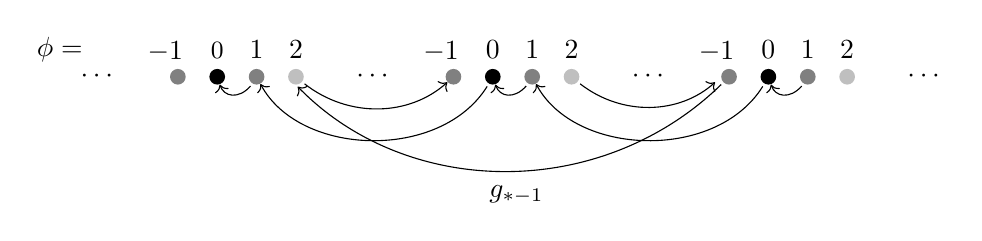
\begin{tikzpicture}

\node at (-5,0) {$\cdots$};
\draw (-4,0) node[circle,fill=gray,inner sep=2pt,label={[xshift=-4.5pt, yshift=-1pt]above: $-1$}] {};
\draw (-3.5,0) node[circle,fill,inner sep=2pt,label={[font=\small]above: $0$}] {};
\draw (-3,0) node[circle,fill=gray,inner sep=2pt,label=above: {$1$}] {} edge[->, bend left=60,looseness=1.5,shorten <=1pt,shorten >=3pt] (-3.5,0);
\draw (-2.5,0) node[circle,fill=lightgray,inner sep=2pt,label=above: {$2$}] {} edge[->, bend right=40,shorten <=1pt,shorten >=3pt] (-0.5,0);

\node at (-1.5,0) {$\cdots$};
\draw (-0.5,0) node[circle,fill=gray,inner sep=2pt,label={[xshift=-4.5pt, yshift=-1pt]above: $-1$}] {};
\draw (0,0) node[circle,fill,inner sep=2pt,label=above: {$0$}] {}  edge[->, bend left=60,shorten <=1pt,shorten >=3pt] (-3,0);
\draw (0.5,0) node[circle,fill=gray,inner sep=2pt,label=above: {$1$}] {} edge[->, bend left=60,looseness=1.5,shorten <=1pt,shorten >=3pt] (0,0);
\draw (1,0) node[circle,fill=lightgray,inner sep=2pt,label=above: {$2$}] {}  edge[->, bend right=40,shorten <=1pt,shorten >=3pt] (2.9,0);
\node at (2,0) {$\cdots$};

\draw (3,0) node[circle,fill=gray,inner sep=2pt,label={[xshift=-4.5pt, yshift=-1pt]above: $-1$}] {} edge[->, bend left=45,shorten <=1pt,shorten >=5pt] (-2.6,0);
\draw (3.5,0) node[circle,fill,inner sep=2pt,label=above: {$0$}] {} edge[->, bend left=60,shorten <=1pt,shorten >=3pt] (0.5,0);
\draw (4,0) node[circle,fill=gray,inner sep=2pt,label=above: {$1$}] {} edge[->, bend left=60,looseness=1.5,shorten <=1pt,shorten >=3pt] (3.5,0);
\draw (4.5,0) node[circle,fill=lightgray,inner sep=2pt,label=above: {$2$}] {};
\node at (5.5,0) {$\cdots$};

\node at (-5.5,0.35) {$\phi=$};
\node at (0.3,-1.5) {$g_{*-1}$};

\end{tikzpicture}
\end{center}

Now, by sending an upper set of $I \in O(\mathbb{Z})$ to its characteristic function $\chi_I$ we get an embedding $$O(\mathbb{Z})^{\textnormal{op}} \hookrightarrow \Xi$$ and the t-structure coming from $(g_{\chi_I})_{\textnormal{\Libra}}(\mathscr{Q})$ is just the tilting of $\mathfrak{t}$ with respect to the torsion pair coming from $I$. \\
The following proposition gives a characterization of the new heart obtained by the above construction. In the case of a mixed filtration, we get a splitting property which is often referred as 'decomposition theorem for perverse sheaves' in literature. \\

\begin{prop}
Let $\mathfrak{t}$ be a bounded t-structure on $\mathscr{D}$, $\mathscr{P}$ a grading filtration on $\heartsuit_{\mathfrak{t}}$, $\mathscr{Q}$ the associated $\mathbb{Z} \ltimes \hat{\mathbb{Z}}$-slicing on $\mathscr{D}$, $p$ a perversity. Denote $\mathfrak{q}$ the bounded t-structure associated to $(g_p)_{\textnormal{\Libra}}(\mathscr{Q})$. Then $\heartsuit_{\mathfrak{q}}$ consists of objects $X \in \mathscr{D}$ so that $$H_{\mathfrak{t}}^{k}(X) \in \mathscr{P}_{p^{-1}(-k)}[k]$$ 
for each $k \in \mathbb{Z}$. Moreover, if $\mathscr{P}$ is a mixed filtration then for each $X \in \heartsuit_{\mathfrak{q}}$ $$X=\bigoplus_{n \in \mathbb{Z}}H_{\mathfrak{t}}^{n}(X)$$ 
\end{prop}

\begin{proof}
This is very similar to \hyperref[tilt1]{\textbf{Proposition \ref*{tilt1}}}: we have that $X \in \heartsuit_{\mathfrak{q}}$ if and only if $$H_{\mathscr{P}}^{\phi}(H_{\mathfrak{t}}^k(X)[-k])[k]=H_{\mathscr{Q}}^{(k,\phi)}(X)=0$$ 
for $p(\phi) \not = -k$. \\
For the second part of the claim, the abelian $\mathbb{Z}$-slicing induced on $\heartsuit_{\mathfrak{q}}$ is split by \hyperref[grad]{\textbf{Proposition \ref*{grad}}} and thus by \hyperref[split]{\textbf{Proposition \ref*{split}}} $$X=\bigoplus_{(k,\phi)}H_{\mathscr{Q}}^{(k,\phi)}(X)=\bigoplus_{n \in \mathbb{Z}}H_{\mathfrak{t}}^{n}(X)$$
where the last equality comes from the first part. 
\end{proof}

\begin{exmp}
Let $$B=\bigoplus_{i\in \mathbb{N}}B_i$$ be an $\mathbb{N}$-graded ring with $B_0$ semisimple. Denote $\mathscr{A}$ the category of $\mathbb{Z}$-graded $B$-modules with only finitely many nonzero graded pieces. For $\phi \in \mathbb{Z}$, denote $\mathscr{P}_{\phi}$ the full subcategory of $\mathscr{A}$ of modules concentrated in degree $\phi$. Clearly, $\mathscr{P}$ defines an abelian $\mathbb{Z}$-slicing on $\mathscr{A}$. Following \cite{kos} we have $$\textnormal{Ext}_{\mathscr{A}}^n(\mathscr{P}_{\phi},\mathscr{P}_{\psi})=0$$
for $n>\psi - \phi$. This means that $\mathscr{P}$ is a mixed filtration and the bounded t-structure on $\mathscr{D}^b(\mathscr{A})$ associated to $(g_1)_{\textnormal{\Libra}}(\mathscr{Q})$ (where $1$ is the identity of $\mathbb{Z}$) is the 'diagonal' (or 'geometric') t-structure which appears in Koszul duality and other areas. 
\end{exmp}

\begin{exmp}
Let $M$ be an $n$-dimensional smooth complex projective variety and consider the $n$-torsion pair $\mathscr{P}$ on $\textnormal{Coh}(M)$ from \hyperref[cohh]{\textbf{Example \ref*{cohh}}}. Using Serre duality and the Grothendieck vanishing theorem, one sees that $\mathscr{P}$, seen as an abelian $\mathbb{Z}$-slicing via the inclusion $[n] \subseteq \mathbb{Z}$, is a perverse filtration. The bounded t-structure associated to $(f_p)_{\textnormal{\Libra}}(\mathscr{Q})$ is the one of perverse coherent sheaves as constructed in \cite{bez}. Following again the proof of \hyperref[t]{\textbf{Proposition \ref*{t}}}, we can use the Harder-Narasimhan filtrations from Gieseker stability to obtain an abelian $J_n$-slicing on the heart of perverse coherent sheaves as done in \cite{perpol}. 
\end{exmp}

Now we somehow review the gluing construction for t-structures in \cite{del}, but generalize it to any slicing. Our language is quite different though, and we formulate the problem very similarly to \cite{glu}. We start with two $\mathbb{Z}$-posets $J,J'$. 

\begin{defn}
Let $\mathscr{P}$ be a $J \ltimes J'$-slicing on $\mathscr{D}$. We call $\mathscr{P}$ \textbf{gluable} if it satisties the assumptions of \hyperref[pipp]{\textbf{Proposition \ref*{pipp}}} with respect to the map $J \ltimes J' \overset{e}{\longrightarrow} J' \ltimes J$ that exchanges coordinates. In this case we denote $$\overline{\mathscr{P}}=e_{\textnormal{\Libra}}(\mathscr{P})$$
\end{defn}

By a simple computation, the gluability condition reads: $\mathscr{P}_{(\phi,\psi)} \subseteq \mathscr{P}_{(\phi',\psi')}^{\perp}$ if $\psi' > \psi$ or both $\psi'+1>\psi$ and $\phi'+1 < \phi$. For example, the first condition is automatic when $\mathbb{Z}$ acts trivially on $J$ (in this case, it follows from the second one). In particular, if $\mathbb{Z}$ acts trivially on $J$, $\mathscr{P}$ is a $J$-slicing on $\mathscr{D}$ and $\mathfrak{t}_{\phi}$ is a bounded t-structure on $\mathscr{P}_{\phi}$ for each $\phi \in J$, then using \hyperref[aab]{\textbf{Proposition \ref*{aab}}} we get a $J \ltimes \mathbb{Z}$-slicing $\mathscr{Q}$ which is gluable if and only if $$\heartsuit_{\mathfrak{t}_{\psi}}[n] \subseteq \heartsuit_{\mathfrak{t}_{\phi}}^{\perp}$$
whenever both $n \le 0$ and $\phi < \psi$. 

\begin{rem}
We have a commutative diagram of $\mathbb{Z}$-posets 
\begin{center}
\begin{tikzcd}[ampersand replacement=\&]
\mathbb{Z} \ltimes \mathbb{Z} \arrow{r}{\sim} \arrow{d}{e} \& \mathbb{Z} \ltimes \hat{\mathbb{Z}} \arrow{d}{g} \\
\mathbb{Z} \ltimes \mathbb{Z} \arrow{r}{\sim}  \& \mathbb{Z} \ltimes \hat{\mathbb{Z}} 
\end{tikzcd}
\end{center}
where the horizontal isomorphism is the one from \hyperref[zet]{\textbf{Remark \ref*{zet}}}. Indeed, a $\mathbb{Z} \ltimes \mathbb{Z}$-slicing on $\mathscr{D}$ is gluable if and only if it induces a grading filtration on the heart of the associated t-structure when seen as a $\mathbb{Z} \ltimes \hat{\mathbb{Z}}$-slicing. 
\end{rem} 

An easy combinatorial calculation finally yelds the following two remarks: 
\begin{itemize}
\item  if $\mathscr{P}$ is a gluable $\hat{\mathbb{Z}} \ltimes \mathbb{Z}$-slicing on $\mathscr{D}$, then $\overline{\mathscr{P}}$ induces a grading filtration on the associated heart, allowing us again to construct new bounded t-structures depending on a perversity. 
\item if $\mathscr{P}$ is a mixed filtration on the heart of a bounded t-structure and $\mathscr{Q}$ is the associated $\mathbb{Z} \ltimes \hat{\mathbb{Z}}$-slicing on $\mathscr{D}$, then $\mathscr{Q}$ is gluable. In this case, looking at $\overline{\mathscr{Q}}$, we get a baric structure on $\mathscr{D}$ which is usually called \textbf{weight decomposition} in literature. 
\end{itemize}
In other words, the chain of implications for a $\mathbb{Z} \ltimes \hat{\mathbb{Z}}$-slicing refines to 
$$\textnormal{mixed} \implies \textnormal{gluable} \implies \textnormal{grading} \implies \textnormal{perverse} $$

%\begin{prop}
%A $J \ltimes J'$-slicing $\mathscr{P}$ on $\mathscr{D}$ is gluable if and only if it satifies the assumptions of \hyperref[pipp]{\textbf{Proposition \ref*{pipp}}} with respect to the identity (as sets) $J \ltimes J' \longrightarrow J \times J'$, where we place the product order on the right member. 
%\end{prop}
%
%\begin{proof}
 % Consider the following commutative diagram of sets
 % \begin{center}
%\begin{tikzcd}[ampersand replacement=\&]
%J \ltimes J' \arrow{r}{e} \arrow{d}{1} \& J \ltimes J' \\
%J \times J' \arrow{r}{e}  \& J \times J' \arrow{u}{1}
%\end{tikzcd}
%  \end{center}
%  The right arrow is a morphism of $\mathbb{Z}$-posets while the down one is an isomorphism of $\mathbb{Z}$-posets, and the thesis follows. 
%\end{proof}
%\begin{prop}
%Let $\mathscr{P}$ be a gluable $J \times J'$-slicing on $\mathscr{D}$. For $i = 1,2$, denote $\mathscr{P}^i=\pi_{\textnormal{\Libra}}^i(\mathscr{P})$, where $J \overset{\pi^1}{\longleftarrow} J \times J' \overset{\pi^2}{\longrightarrow} J'$ are the projections. Then for each $\psi \in J'$, $\mathscr{P}_{\psi}^2$ consists of objects $X \in \mathscr{D}$ so that $$H_{\mathscr{P}^1}^{\phi}(X) \in \mathscr{Q}_{(\phi,\psi)}$$
%for each $\phi \in J$.
%\end{prop}
%
%\begin{proof}
%We have already seen that $X \in \mathscr{P}_{\psi}^2$ if and only if $$H_{\mathscr{P}}^{\lambda}(X)=H_{\mathscr{P}}^{\lambda}(H_{\mathscr{P}^1}^{\pi^1(\lambda)}(X))=0$$
%for $\pi^2(\lambda) \not =\psi$. By fixing $\pi^1(\lambda)=\phi$ and varying $\pi^2(\lambda)$, we get the desired result. 
%\end{proof}
\newpage



\afterpage{\blankpage}
\clearpage 
\bibliographystyle{alpha}


\end{document}

 


